% !Mode:: "TeX:UTF-8"
% !TEX builder = LATEXMK
% !TEX program = xelatex
\documentclass[master, oneside]{hduthesis} % 如果你的论文不满80页,还是单面印刷吧

\usepackage{graphicx}%插图宏集
\usepackage{titletoc}%要调整章节标题在目录页中的格式,可以用titletoc宏包 title of contents
\usepackage{titlesec} %其中 center 可使标题居中,还可设为 raggedleft (居左,默认),
%\usepackage{abstract}摘要分栏的宏包
\usepackage{fontspec, xunicode, xltxtra}
\usepackage{xeCJK}%中文字体

%%%%%%%%%%%%%%%%%%%%%%%%%%%%%% 开始填写前置部分使用的变量
%%%%%%%%%%%%%%%%%%%%%%%%%%%%%% 样式设定在 zjuthesis.cls 下, 人类可读,爱请查阅

% 这里写这么鬼畜是为了测试多几个字会不会造成溢出
\title{多智能体系统中安全一致性算法的设计与分析} % 封面和题名页使用
\englishtitle{Research on distributed security mechanism of multi-agent system} % 封面和题名页使用
% 如果您的标题用字过多,请自行调节 zjuthesis.cls 里的 ZJUmakecover 里的各项距离。

%\author{伊藤春希}          % 申请人姓名 封面使用
\author{严浩峰}
\englishauthor{Haofeng, Yan}

\classification{TP311.1}    % 封面头使用
\serialnumber{10335}        % 封面头使用
\secretlevel{无}            % 封面头使用
\studentnumber{21x51xxx}    % 封面头使用

%\supervisor{御坂美琴}       % 导师 封面使用
\supervisor{吴铤、徐明}
\englishsupervisor{Ting, Wu}
\englishspvtitle{Professor}           % 职称 封面使用
\cspvtitle{教授}              % 职称 封面使用

% 合作导师,如果没有合作导师,就在此文件第 4 行\documentclass选项栏中加上"nocpsupervisor"。

\spvtitle{教授}             % 合作导师职称

% 从机械工程学院改来,保留设定变量命名
%\major{船舶工程}            % 专业学位类别栏 填 工程硕士
\major{软件工程}
%\research{白学}             % 专业学位领域栏 填 软件工程
\research{软件工程}
\institute{计算机学院}         % 所在学位栏 填 软件学院

\submitdate{2333年2月33日}   % 论文提交日期 栏

% 题名页的评阅人及答辩席
% 归档时候填写
% 论文评阅人1 2 3 4 5
\reviewerA{} \enreviewerA{}
\reviewerB{} \enreviewerB{}
\reviewerC{} \enreviewerC{}
\reviewerD{} \enreviewerD{}
\reviewerE{} \enreviewerE{}

% 答辩委员会主席
\chairperson{} \enchairperson{}

% 答辩委员 1 2 3 4 5
\commissionerA{} \encommissionerA{}
\commissionerB{} \encommissionerB{}
\commissionerC{} \encommissionerC{}
\commissionerD{} \encommissionerD{}
\commissionerE{} \encommissionerE{}

% 答辩日期
\defencedate{2018年7月} \eendefencedate{July, 2018}  % 因为endefencedate 命名被占用

% 论文前置部分变量填写完毕 开始全书排版
\begin{document}

% 封面、中文题名页、英文题名页、独创声明和版权使用书 无页码
\maketitle

% 摘要部分
\abstractmatter
% !TEX root = ../main.tex

% 定义中文摘要和关键字
\begin{cabstract}
本文的目的是区分数码相机拍摄的自然图像(NI)和计算机图形渲染软件创建的计算机生成的图形(CG)。本文的主要贡献有三个。首先,我们提出利用两个不同的去噪滤波器来获取检测图像的一阶和二阶噪声,并假设残差噪声遵循所提出的统计模型来分析其特性。其次,在假设检验理论框架下,将NI与CG之间的识别问题顺利转移到似然比检验(LRT)的设计中,同时了解所有的干扰参数,同时从理论上考察LRT的性能。第三,在实际分类中,使用估计的模型参数,我们建议建立一个广义似然比检验(GLRT)。模拟和真实数据的大规模实验结果直接验证了我们提出的测试能够从NI中识别具有高检测性能的CG,并且显示出与一些现有技术相当的效果。此外,通过考虑一些后处理技术产生的攻击来验证所提出的分类器的鲁棒性。

\end{cabstract}

\ckeywords{自然图像,计算机生成的图形,数字图像取证,统计噪声模型,假设检验}

% !TEX root = ../main.tex

% 定义英文摘要和关键字

\begin{eabstract}
The purpose of this paper is to differentiate between natural images (NI) acquired by digital cameras and computer- generated graphics (CG) created by computer graphics rendering software. The main contributions of this paper are threefold. First, we propose to utilize two different denoising filters for acquiring the first-order and second-order noise of the inspected image, and analyze its characteristics with assuming that residual noise follows the proposed statistical model. Second, under the framework of the hypothesis testing theory, the problem of identifying between NI and CG is smoothly transferred to the design of the likelihood ratio test (LRT) with knowing all the nuisance parameters, and meanwhile the performance of the LRT is theoretically investigated. Third, in the practical classification, using the estimated model parameters, we propose to establish a generalized likelihood ratio test (GLRT). A large scale of experimental results on simulated and real data directly verify that our proposed test has the ability of identifying CG from NI with high detection performance, and show the comparable effectiveness with some prior arts. Besides, the robustness of the proposed classifier is verified with considering the attacks generated by some post-processing techniques.
\end{eabstract}

\ekeywords{Natural image, computer-generated graphic, digital image forensics, statistical noise model, hypothesis testing}


% 目录和术语表
%\frontmatter
\tableofcontents % 正文目录
%\listoffigures   % 图目录
%\listoftables    % 表目录
% 术语及缩略词表(需要则开)
%\include{contents/denotation}

% 正文排版开始 建议一章一编辑 (好像无法嵌套 include)
\mainmatter
% !TEX root = ../main.tex

% 第一章一般名为绪论/引言,不可省略

\chapter{绪论}

\section{研究背景与意义}


\section{国内外研究现状}

\section{论文研究内容}

\section{论文组织结构}

简明扼要的介绍下各章主旨,版面控制半页内。
 % 绪论
%!TEX root = ../main.tex

\chapter{分布式一致性算法的介绍}
% 原则上,每一章开头不可马上进入第一节
% 需要一段引文提要起到 TL;DR 的作用

\section{图论知识}

\subsection{矩阵理论}


\section{分布式一致性算法及其安全性}

\section{MSR家族算法的相关研究}





%!TEX root = ../main.tex
\chapter{基于移动辅助节点的MSR一致性算法}

\section{引言}

\section{问题描述}

\subsection{网络模型}

\subsection{一致性算法介绍}

\subsection{目标问题}

\section{移动辅助下的MSR算法设计及分析}

\subsection{移动模型}

\subsection{一致性协议}

\subsection{实现一致性分析}

\section{仿真实验与结果分析}

\section{本章小结}


%\chapter{在一般网络中的基于移动探测器的MSR一致性算法}
\chapter{基于最大一致性的弹性时钟同步算法}

\section{引言}

\section{问题描述}

\subsection{时钟模型}

\subsection{网络模型与攻击介绍}

\subsection{问题设置}

\section{分布式时钟同步算法的设计}

\subsection{相对斜率估计}

\subsection{最大一致性下的弹性斜率补偿}

\subsection{最大一致性下的弹性偏差补偿}

\section{仿真实验与结果分析}

\section{本章小结}

%!TEX root = ../main.tex

\chapter{总结和展望}

\section{相关工作总结}

本模板主要内容来源于ZJU-Awesome项目,
参考软件学院论文格式要求做出调整,
并加入补充宏包,调整若干属性配置完成。
封面方面主要调整了各栏间距和对齐,
摘要依照软件学院更改了关键字的样式和页码的样式。
软件学院规定从摘要起每页必须有对应章标题的页眉,
虽然在一般排版习惯里,章头处不应设置页眉,
但考虑到已有大部分同学使用Word字处理软件遵照执行,
为保一致性,本模板暂时向软件学院的设定妥协。
由于论文格式要求并未向章头处的间距做出任何设定,
本模板保留ZJU-Awesome设定。
除此之外,本模板还做出了不少微小的改动。
详情请仔细阅读\texttt{zjuthesis.cls}和\texttt{main.tex}相关内容。

考虑到大部分软件学院的同学对\LaTeX 论文排版的陌生,
本文以尽量精炼的篇幅介绍了论文排版工作的各方面。
现在给出一个参考流程如\autoref{fig:workflow} 希望能对初次使用
\LaTeX 排版论文的同学一点提示。

\begin{figure}[htbp]
    \centering
    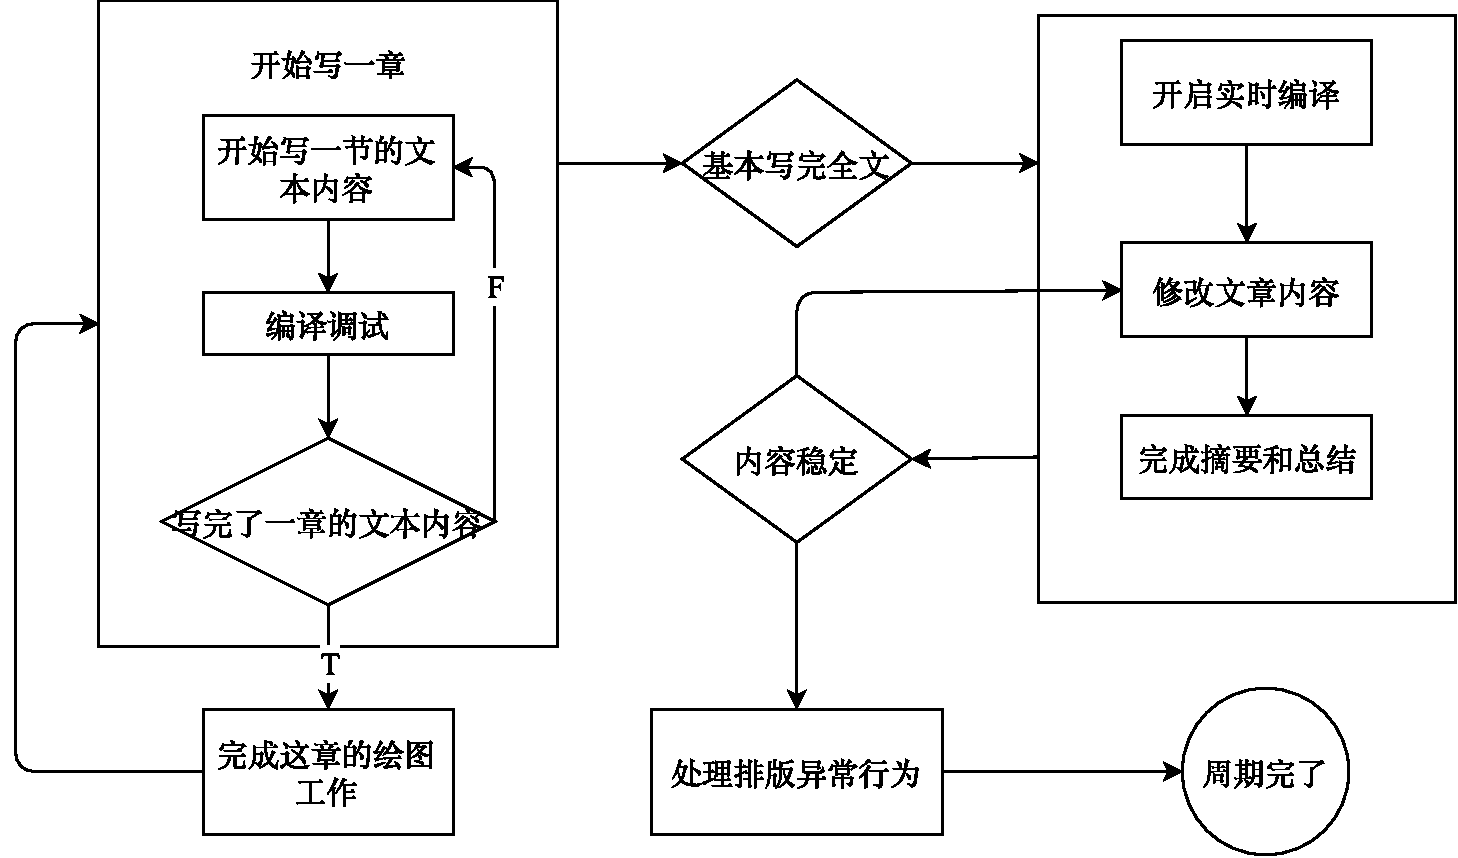
\includegraphics[width=.8\textwidth]{workflow.pdf}
    \caption{论文排版工作参考流程}
    \label{fig:workflow}
\end{figure}

\section{研究工作展望}

本文没有讨论各式\LaTeX 环境的使用细则,宏包的具体细节,
调试查错的技巧,也几乎没有交待任何一种具体的绘图方案。
希望屏幕前的你能以最少的代价完成论文排版工作,
养成内容和样式分离的电子写作习惯,
并能独立思考信息表达的最佳模式。

本文草拟于2016年夏季毕业论文送审前,
希望本文能抛砖引玉,
对\LaTeX 有经验的后辈们若能继续完善甚至颠覆本模板的设定,
相信一定能对软件学院的论文排版素质起到根本的改善作用。
  % 总结和展望

% 结尾部分排版
\backmatter

% 引用参考文献数据库
\bibliography{references/test.bib}

% 附录部分
%\appendix
\include{contents/appendixA}

% 作者简历
%% !TEX root = ../main.tex
\chapter{作者简历}
\noindent 教育经历:

\begin{tabular}{llll}
    2014年9月至2016年6月: &  浙江大学  & 软件工程  &  硕士    \\
    2010年9月至2014年6月: &  三墩工学院  & 电脑挖掘机维修  &  混混
\end{tabular}

\noindent 工作经历:

\begin{tabular}{llll}
    2015年6月至2016年3月: &  FLAG   &  码畜
\end{tabular}

% \noindent 攻读学位期间发表的论文或研究成果:



% 致谢
% 致谢不必感谢在下,
% 但请一定感谢清华大学薛瑞尼、
% 浙江大学机械工程学院陈九历
%% !TEX root = ../main.tex
\chapter{致\ZJUspace{}谢}

在去年撰写开题报告和文献综述时,
搜索Github发现了仅在数月前发布的ZJU-Awesome项目。
简单套用后自觉此法应当推广。
于是在2016年3月撰写论文结束后,
下决心向软件学院的同学推广此一模板,
继而有了本文和在下对模板的调整。

衷心感谢ZJU-Awesome项目作者之一机械工程学院的陈九历同学耐心解答在下的多次疑问。

% 难道不应该感谢世界(大雾)
也感谢夏目友人帐能让我在论文写作过程中保持着一份平静,
最后感谢这份文稿前的你,能仔细阅读到这一页。

\vspace{2cm}
\hfill
\begin{minipage}{14em}
    \begin{flushright}
        君之名\\
        %于浙江大学软件学院\\ % 学院要求的格式 - -#
        %2016年4月18日   % 与封面论文提交时间一致
        2017年1月1日\\
        于老和山下
    \end{flushright}
\end{minipage}


\end{document}
